\documentclass[11pt]{article}
\usepackage{amsfonts}
\usepackage{amsmath}
\usepackage{amsthm}
\usepackage{amssymb}
\usepackage{mathrsfs}
\usepackage[fit]{truncate}
\usepackage{acl2012}
\usepackage{times}
\usepackage{latexsym}
\usepackage{amsmath}
\usepackage{url}
\usepackage{graphicx}
\usepackage{caption}
\usepackage{multirow}
\usepackage{dblfloatfix}
\usepackage{float}
\usepackage{subfigure}
\DeclareMathOperator*{\argmax}{arg\,max}
\setlength\titlebox{5.2cm}    % Expanding the titlebox



\newcommand{\affliationPenn}{\ensuremath{{}^\text{1}}}
\newcommand{\affliationJHU}{\ensuremath{{}^\text{2}}}

\title{A large scale study of the languages spoken (by bilinguals) on Mechanical Turk}
\title{The Language Demographics of  Amazon Mechanical Turk}

\author{Ellie Pavlick\affliationPenn \ \ \ \ \ \ \ \ \ \ Dmitry Kachaev\affliationJHU \ \ \ \ \ \ \ \ \ \  Chris Callison-Burch\affliationPenn$^{,}$\affliationJHU \\
\affliationPenn Computer and Information Science Department, University of Pennsylvania \\
\affliationJHU Human Language Technology Center of Excellence, Johns Hopkins University \\
  }

\date{}

\begin{document}
\maketitle

\begin{abstract}
We present a large scale study of the languages spoken by bilingual workers on Mechanical Turk (MTurk).  
We establish a  methodology for determining the language skills of anonymous crowd workers that is more robust than simple surveying.  We validate workers' self-reported language skill claims by measuring their ability to correctly translate words, and by geolocating workers to see if they reside in countries where the languages are likely to be spoken. Rather than posting a one-off survey, we posted paid tasks consisting of 1,000 assignments to translate a total of 10,000 words in each of 119 languages.  Our study ran for weeks, and was highly visible on the MTurk crowdsourcing platform, increasing the chances that bilinguals workers would complete it.  Our study was useful both to create bilingual dictionaries and to act as census of the bilingual speakers on MTurk.  We use this data to recommend languages with the largest speaker populations as good candidates for other researchers who want to  develop crowdsourced, multilingual technologies.

\end{abstract}

\section{Overview}
Crowdsourcing is a promising new mechanism for collecting data for natural language processing research. Access to a fast, cheap, and flexible workforce allows us to collect new types of data, potentially enabling new language technologies.
Because crowdsourcing platforms like Amazon Mechanical Turk (MTurk) give researchers access to a worldwide workforce, one obvious application of crowdsourcing is the creation of multilingual technologies. 
With an increasing number of active crowd workers located outside of the United States, there is even the potential to reach fluent speakers of lower resource languages.
In this paper, we investigate the feasibility of hiring language informants on MTurk by conducting the first large-scale demographic study of the languages spoken by workers on the platform. 

%Access to a fast, cheap, and flexible workforce has changed the way we collect data, and holds promise for enabling future language technologies. Crowdsourced work has proven effective for collecting massive amounts of simple data annotations, such as annotating data for face recognition software and labeling sentiment in twitter data. As the demands and expectations of automated systems progress, and the complexity of the data required for training increases, however, it becomes natural to ask about the strengths and limitations of the crowd as annotators for natural language data.
%We evaluate the language skills of bilingual workers on Amazon's Mechanical Turk, and their ability to provide translated data for statistical machine translation. Collecting parallel translated texts has traditionally been assumed to require a higher level of expertise than what is available from non-professional crowd workers. However, with an increasing number of active crowd workers located outside of the United States, the potential to access fluent speakers of lower resource languages makes crowdsourcing an attractive resource for translation.

There are several complicating factors when trying to take a census of workers on MTurk.  The workers identities are anonymized, and Amazon provides no information about their countries of origin nor their language abilities.  Posting a simple survey to have workers self-report this information may be inadequate, since (a) many worker may never see the survey, (b) many opt not to do one-off surveys since potential payment is low, and (c) validating the answers of respondents is not straightforward. 

Our study establishes a methodology for determining the language demographics of anonymous crowd workers that is more robust than simple surveying. We ask workers what languages they speak and in what country they reside, and validate their claims by measuring their ability to correctly translate words and by geolocating them.  To increase the visibility and the desirability of our tasks, we post 1,000 assignments in each of 119 languages.  These tasks each consist of translating 10 foreign words into English.  Two of the 10 words have known translations, allowing us to validate the the workers' translations are accurate, while constructing bilingual dictionaries with up to 10,000 entries, with the majority of entries being new. 

Surveying thousands of workers allows us to analyze current speaker populations for more than 100 languages.  The data also allows us to answer questions like: 
How quickly is work completed in a given language? 
Are crowdsourced translations reliably good? 
How often do workers misrepresented their language abilities to 
%falsely
obtain financial rewards? 


%%%%%%%%%%%%%%% NAT LANG PIE %%%%%%%%%%%
\begin{figure*}[h]
\centering
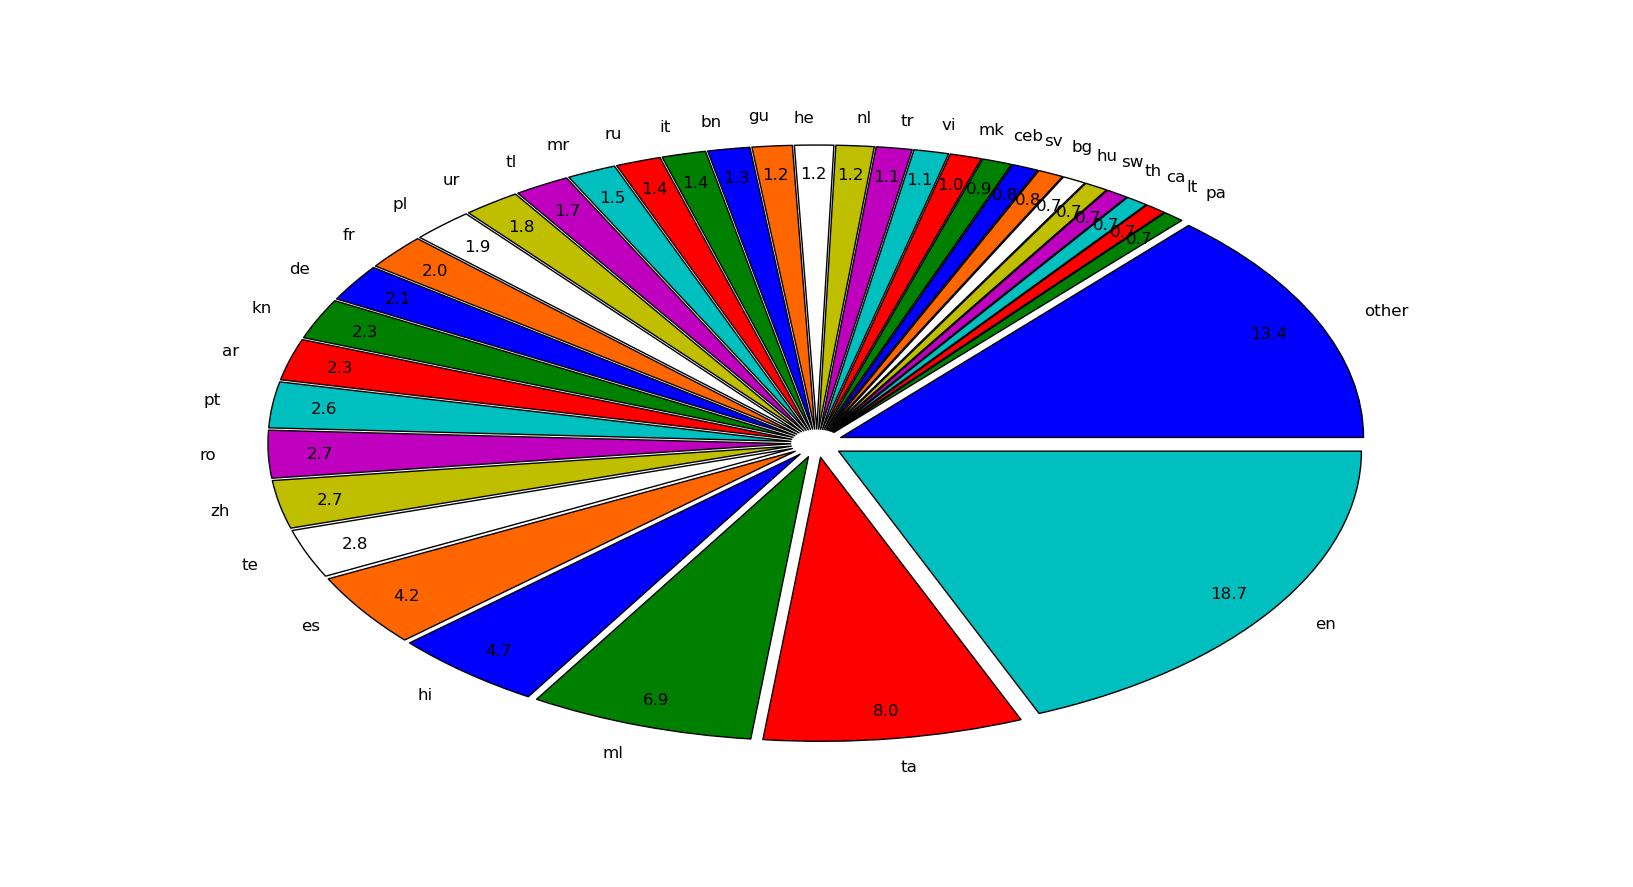
\includegraphics[width=7in]{figures/natlang-pie}
\caption{Self-reported native language of 3154 bilingual turkers}
\label{lang-pie}
\end{figure*}
%%%%%%%%%%%%%%%%%%%%%%%%%%%%%%%%%%%%%%%

%%%%%%%%%%%%%%% NAT LANG PIE %%%%%%%%%%%
\begin{figure*}[h]
\centering
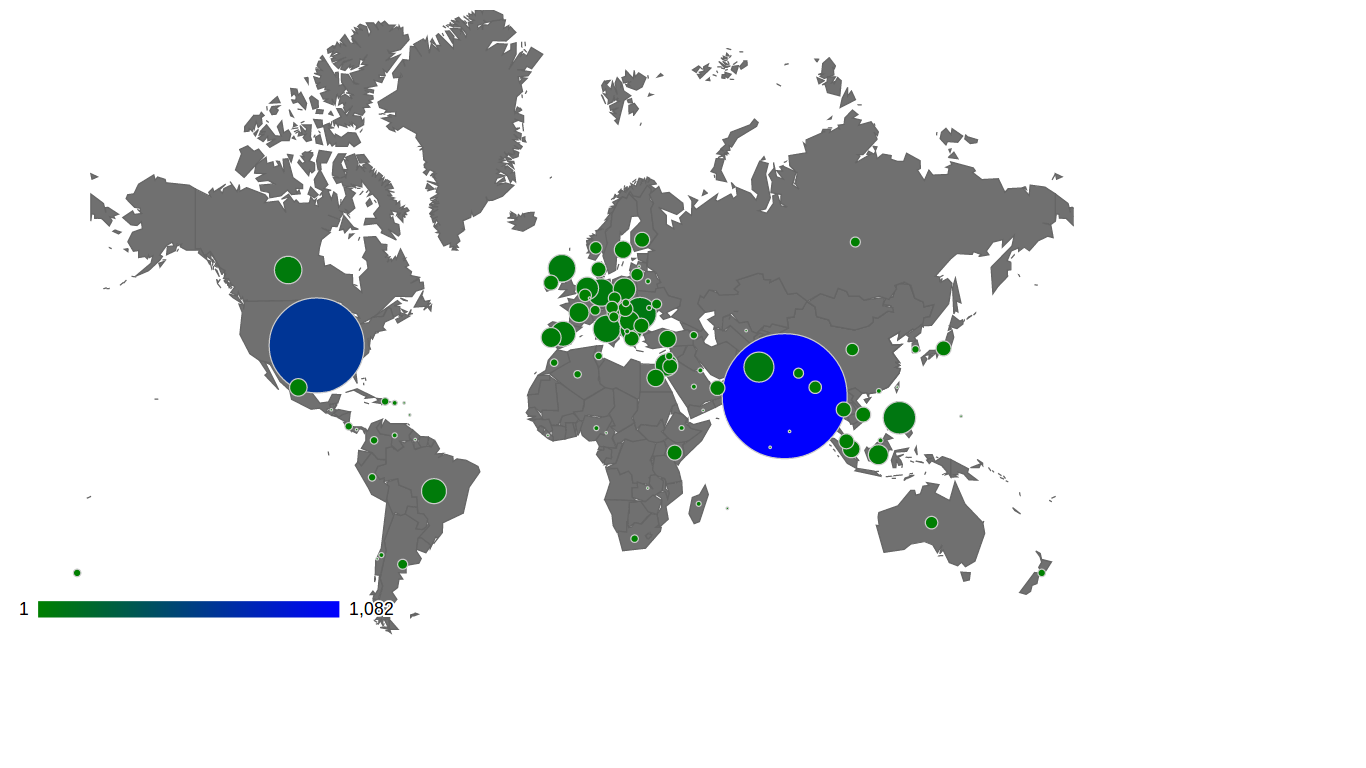
\includegraphics[width=7in]{figures/turkermap-color}
\caption{}
\label{map}
\end{figure*}
%%%%%%%%%%%%%%%%%%%%%%%%%%%%%%%%%%%%%%%

\section{Background and Related Work}
%\section{Background on Mechanical Turk and Related Work}
%\section{Mechanical Turk}
Amazon's Mechanical Turk (MTurk) is an online marketplace for work which gives employers and researchers access to a large, low-cost, human workforce. MTurk provides a simple interface for accessing human skill, allowing requesters to provide micro-payments in return for workers completing micro-tasks.  The basic units of work on MTurk are called ``Human Intelligence Tasks'' (HITs), which suggests that it was designed to accommodate tasks that are difficult for computers, but simple for people. This allows for research into human computation, where people can be treated as a function call \cite{vonAhn2008,Little2009,quinn-bederson:2011}, as well as for large-scale annotation of training data for machine learning applications, including computer vision \cite{sorkin-forsyth:2008,deng-et-al:2010,rashtchian:10} and natural language processing \cite{Snow2008,callisonburch-dredze:2010:MTURK}. 
%In 2010, NAACL hosted a workshop on Creating Speech and Language Data with MTurk, in which MTurk was used to generate data for 24 different natural language tasks \cite{callisonburch-dredze:2010:MTURK}.

Within MTurk, those who need work completed (`requesters') post individual `Human Intelligence Tasks,' or just `HITs'. A typical HIT  requires a few minutes of work and pays a few cents, although there is significant variation across HITs. Once a HIT is posted, MTurk workers (`Turkers') are free to choose to complete the HITs which interest them. Worker identities remain anonymous to requesters, and all payment occurs through Amazon. Requesters are able to accept submitted work or reject work that they do not feel meets their standards, and only pay workers from whom they accept tasks. 
Several reports examine Mechanical Turk as a marketplace \cite{ipeirotis:2010:marketplace,lehdonvirta-ernkvist:2011}.  When Amazon introduced MTurk, it first offered payment only in Amazon credits, and later offered direct payment in US dollars. More recently has expanded to include one foreign currency, the Indian rupee. Despite its payments being limited to two currencies or Amazon credits, MTurk claims over half a million workers from 190 countries.\footnote{https://requester.mturk.com/tour}  This suggest that it has a diverse worker population that should represent a wide variety of languages.

%Within MTurk, those who need work completed (`requesters') post individual HITs. A typical HIT  requires a few minutes of work and pays a few cents, although there is significant variation across HITs. Once a HIT is posted, MTurk workers (`Turkers') are free to choose to complete the HITs which interest them. Worker identities remain anonymous to requesters, and all payment occurs through Amazon. Requesters are able to accept submitted work or reject work that they do not feel meets their standards, and only pay workers from whom they accepted tasks. 

%The convenience and low cost of using MTurk has made it popular among researchers. Because of the lack of oversight and the high potential for spam, however, most of the data collected from MTurk has been limited to simple tasks for which inter-annotator agreement is expected to be high (see Related Work section below). We explore the idea that MTurk's machinery is flexible enough to support more complex tasks requiring more nuanced quality control mechanisms, which could allow it to be a competitive alternative to professional data annotations.

%\section{Related Work}

Typically, researchers rely on large amounts of MTurk data in order to compensate for the high likelihood of low quality labels. Snow et al. describes the success of using redundant non-expert labels to substitute for professional annotations, achieving comparable quality for much lower cost. The tasks from which these conclusions were drawn, however, were kept simple and easily-verifiable, with annotations restricted to either multiple choice or bounded numeric inputs. As NLP research advances, the level of expertise required from annotators advances as well. Callison-Burch et al. report success using MTurk to build parallel corpora for Machine Translation, a task which requires Turkers to speak two languages with a high level of proficiency.

As the use of MTurk has grown, researchers have become interested in who exactly makes up the Turker population. Early demographic studies by \newcite{ipeirotis:2010:demographics} revealed that Turkers are typically younger and more educated than the population as a whole. The study found that while most Turkers cite money as a motivation for working on MTurk, few cite it as their only motivation. A follow-up study by Ross et al. found that the majority of Turkers were located in the US, 30\% of Turkers were located in India, and that Indian Turkers tend to have lower incomes than US-based Turkers. Ross et al. also suggested that the international presence on MTurk has been growing over time. While there has not yet been a thorough investigation of Turkers' language abilities, \newcite{munro-tily:2011} compiled survey responses of 2,000 Turkers, revealing that four of the six most represented languages come from India (the top six being Hindi, Malayalam, Tamil, Spanish, French, and Telugu). No study has yet been conducted to comprehensively assess the language skills of the growing number of international and bilingual Turkers or to analyze the potential of MTurk to support work in low-resource languages. 


%%%%%%%%%%%%%%% HIT UIs %%%%%%%%%%%
\begin{figure}[h]
\centering
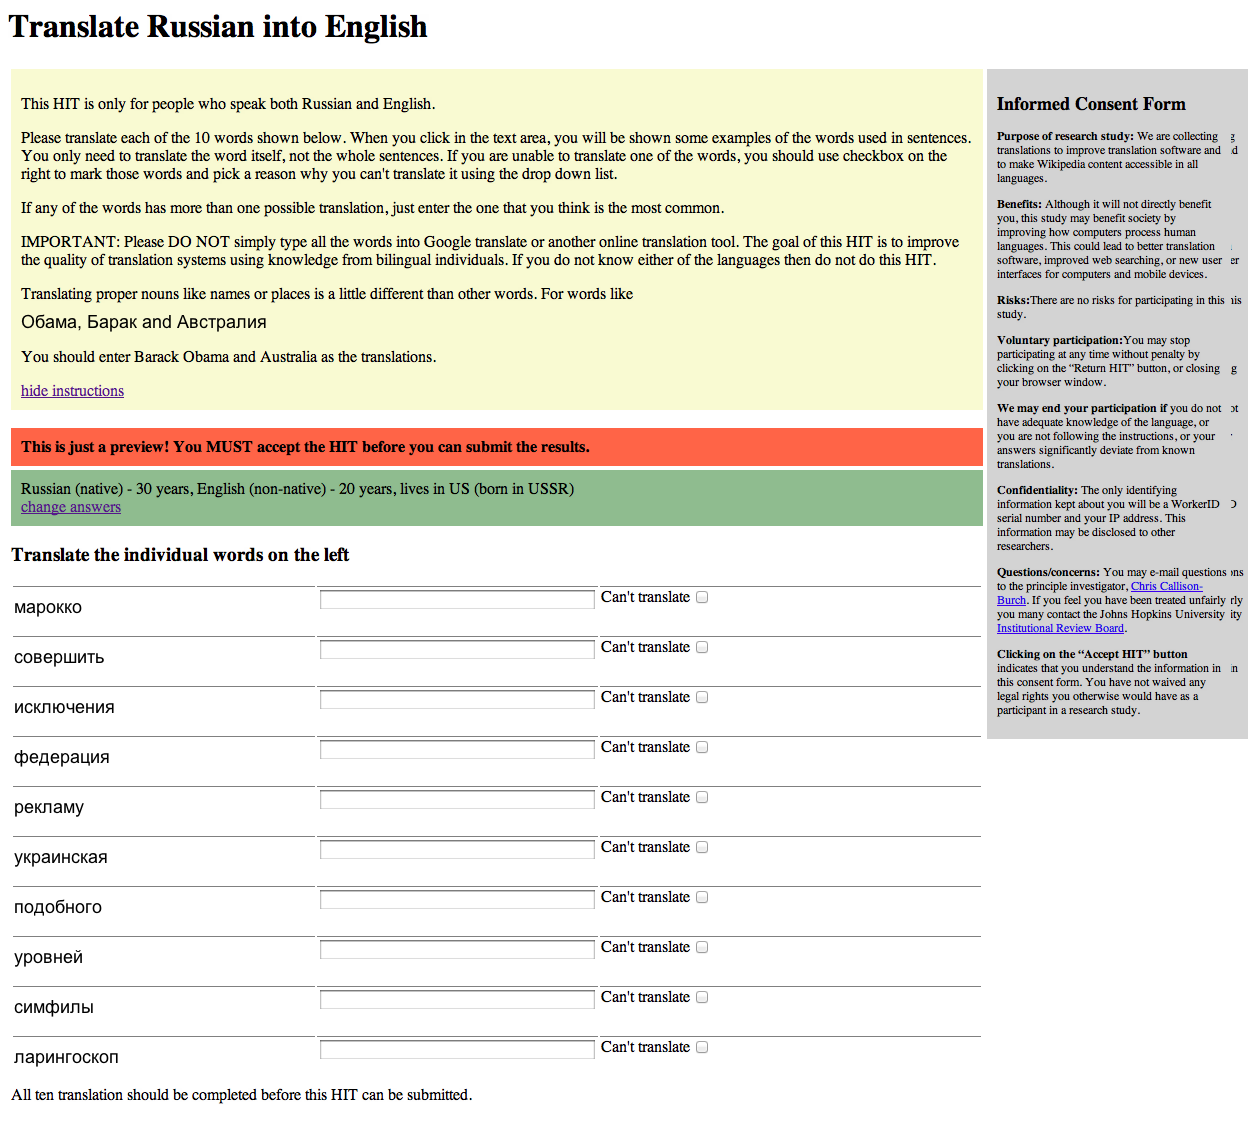
\includegraphics[width=3in]{figures/vocabulary_hit_mturk}
\caption{Translation HIT UI}
\label{tranhit}
\end{figure}

\begin{figure}[h]
\centering
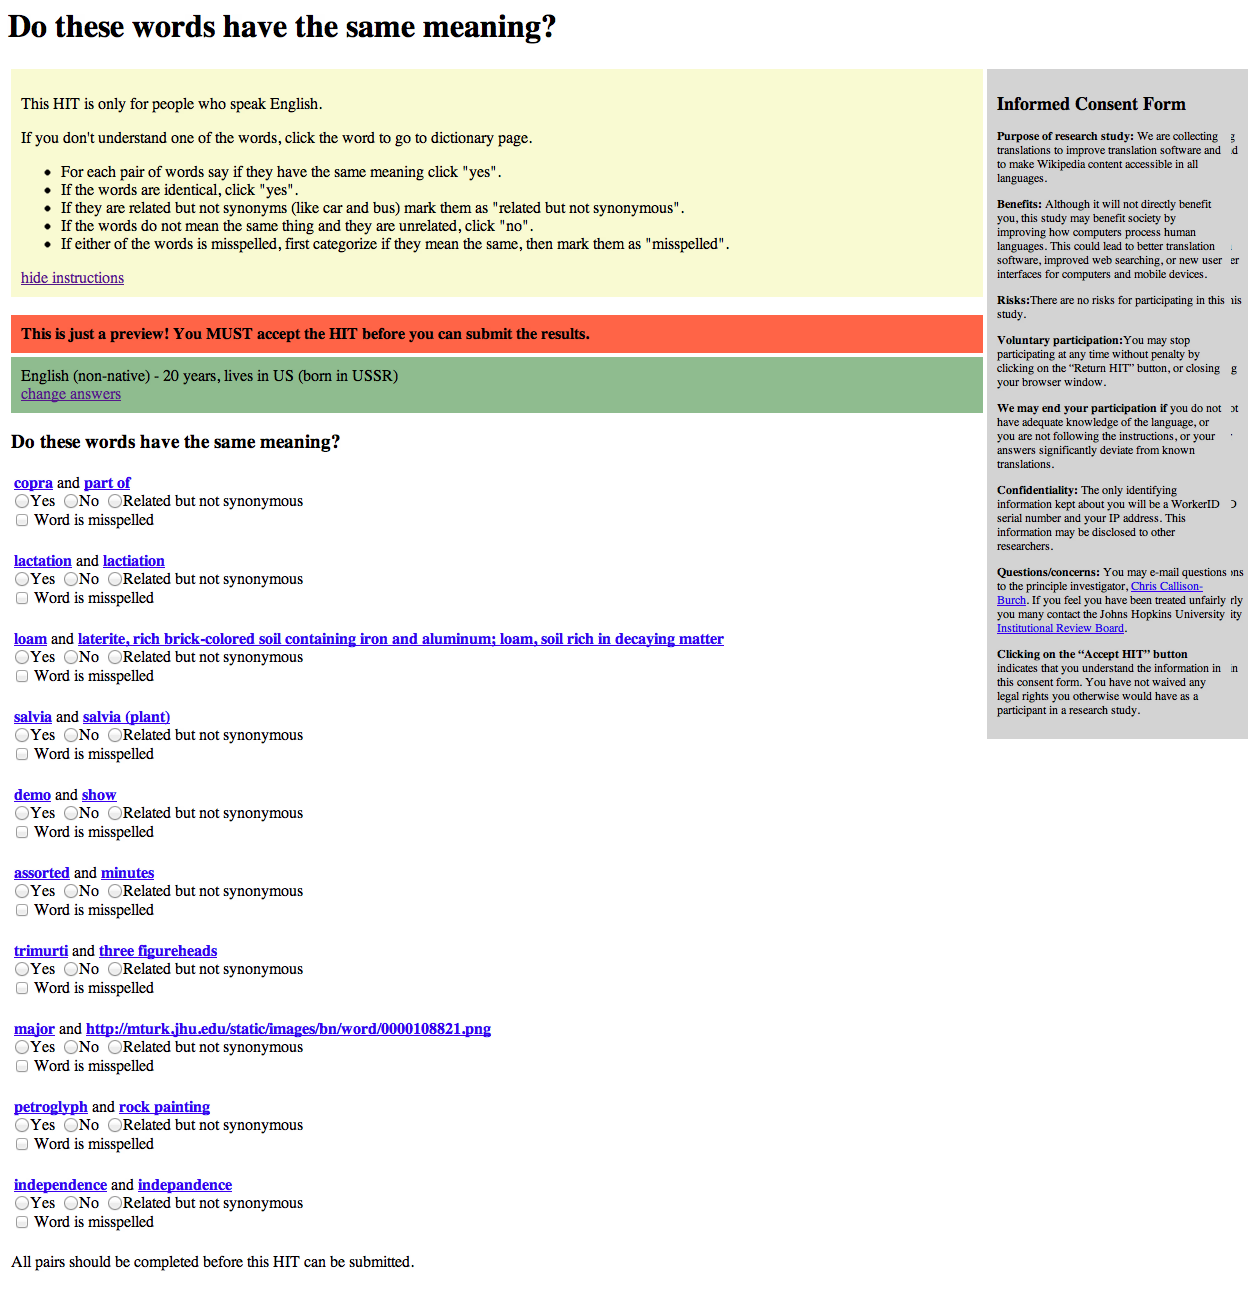
\includegraphics[width=3in]{figures/synonyms_hit_mturk}
\caption{Evaluation HIT UI}
\label{synhit}
\end{figure}
%%%%%%%%%%%%%%%%%%%%%%%%%%%%%%%%%%%%%%%%%%%%%%%%%%%%%%%%

%%%%%%%%%%%%%%% SURVEY TABLE %%%%%%%%%%%
\begin{table*}[h]
\centering
\begin{tabular}{lc}\hline\hline\\
Is [HIT language/English] your native language? &129,049\\
How many years have you spoken [HIT language]?&159,807\\
How many years have you spoken English?&159,808\\
What country do you live in?&329,033\\
Current location (collected automatically)& 329,033\\
\hline\\
Total assignments& 329,033\\
Total unique workers& 6,034\\
\hline\hline
\end{tabular}
\caption{Demographic survey questions and number of assignments with valid responses for each}
\label{survey-tab}
\end{table*}
%%%%%%%%%%%%%%%%%%%%%%%%%%%%%%%%%%%%%%%%%%%%%%%%%%%%%%%%

\section{Task Design}
The central task in this study was to use Mechanical Turk to create low cost, high quality bilingual dictionaries for over 100 languages in order to test the reliability and breadth of the knowledge of Mechanical Turk's bilingual population. 

We chose the languages which were highly used on Wikipedia, in terms of the number of available articles. We compiled a list of all languages for which there existed at least 10,000 Wikipedia articles; we also included a small number of low resource languages for which there were approximately 1,000 available articles, giving a total of 119 languages to use in our task. For each of the languages, we chose the 1,000 most popular articles, and from these selected the 10,000 most frequent words. The resulting vocabularies served as the source side of our dictionaries.

The dictionary creation task was broken into two steps: a translation HIT and an evaluation HIT. Examples of the interface for each are shown in figures \ref{tranhit} and \ref{synhit}.  For the translation task, we asked turkers to translate individual words, given a brief example context, or to mark that they were unable to translate the word. Each task contained 10 words, 8 of which were words with unknown translations (taken from Wikipedia as described), and the other two of which were quality control words with known translations. The task paid one million dollars for the translation of 10 words. 

For the evaluation task, Turkers were shown a pair of words, one which was a Turker's translation of one of the embedded quality control words, and the other which was a known gold-standard translation of the same word. Evaluators were asked whether the two words were synonyms, and chose between three answers: `Yes', `No', or `Related but not synonyms'. The last category was intended for word pairs such as `clouds' and `sky', which may be confusable to a non-native speaker but are not acceptable as dictionary translations. Turkers in the evaluation task could also flag the translated word as misspelled. Each HIT included 10 word pairs to be compared, and paid next to nothing. We describe the evaluation process further in the Measuring Quality section of this paper.

Quality control for the evalutation HIT consisted of embedded word pairs which were either known to be synonyms or were known to be unrelated. Whether the evaluators correctly labeled the known word pairs could be assessed automatically, allowing the evaluation HIT to be the final step of the dictionary creation pipeline.


\section{Turker Demographics}
At the start of each HIT, Turkers were asked to complete a brief survey about their language abilities. Valid responses to all survey questions were not required in order to complete the HIT; survey questions and the number of valid responses received for each are listed in table \ref{survey-tab}. Although it was not required, Turkers who completed multiple HIT assignments could fill out the survey multiple times. This enabled some Turkers to report multiple native languages (see figure \ref{numlangs-tab}). While most results presented are calculated across all Turkers, figures given for distributions across native languages are calculated only from Turkers who reported a single native language.\\

%%%%%%%%%%%%%%% NUM LANGUAGES TABLE %%%%%%%%%%%
\begin{figure}[h]
\begin{tabular}{ccc}\hline\hline
&\# languages&\# Turkers\\ \hline
No languages&0&1801\\
One language&1&3154\\
Multiple languages&2&243	\\
&3&49\\
&4&12\\
&5&9\\
&6&5\\
&7&2\\
&8&1\\
&9&2\\
&10&2\\
&15&1\\
\hline\hline
\end{tabular}
\label{numlangs-tab}
\caption{Number of native languages reported during demographic survey.}
\end{figure}
%%%%%%%%%%%%%%%%%%%%%%%%%%%%%%%%%%%%%%%%%%%%%%%%%%%%%%%%

%%%%%%%%%%%%%%% ASSIGNMENT SCATTER %%%%%%%%%%%
\begin{figure*}[h]
\centering
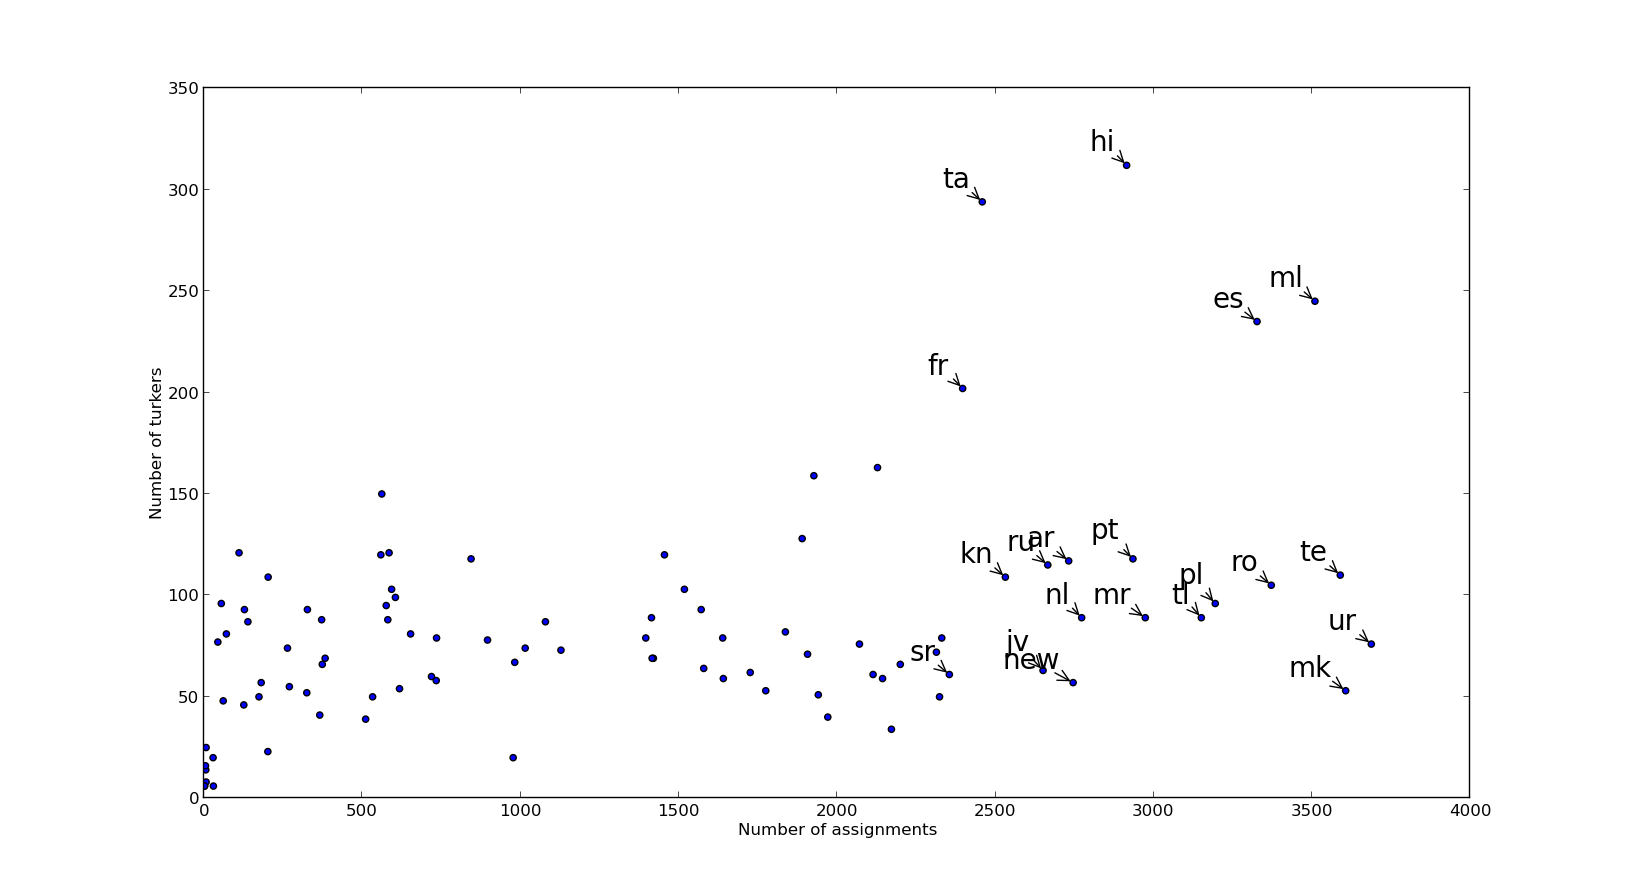
\includegraphics[width=6in]{figures/assign-turk-scatter}
\caption{Number of assignments and number of turkers for each language. Each dot represents a language.}
\label{ass-scatter}
\end{figure*}
%%%%%%%%%%%%%%%%%%%%%%%%%%%%%%%%%%%%%%%%%%%%%%%%%%%%%%%%

Figure \ref{ass-scatter} shows the volume of HITs completed and the number of workers participating for each language. While the bulk (22\%) of bilingual turkers report English as their native language (see figure \ref{lang-pie}), Mechanical Turk's capacity to support the Indian languages is apparent. Hindi, Tamil, and Malayalam are especially well represented in terms of number of active translators, and Urdu, Telugu, and Macedonian are particularly productive in terms of number of assignments completed. As shown in figure \ref{langgeo-bar}, 11 of the top 25 languages, in terms of number of assignments submitted, were Indian languages, and the assignments for 15 of the top 25 were completed mostly or entirely by turkers located in India. 

%%%%%%%%%%%%%%% LOCATION BAR %%%%%%%%%%%
\begin{figure*}[h]
\centering
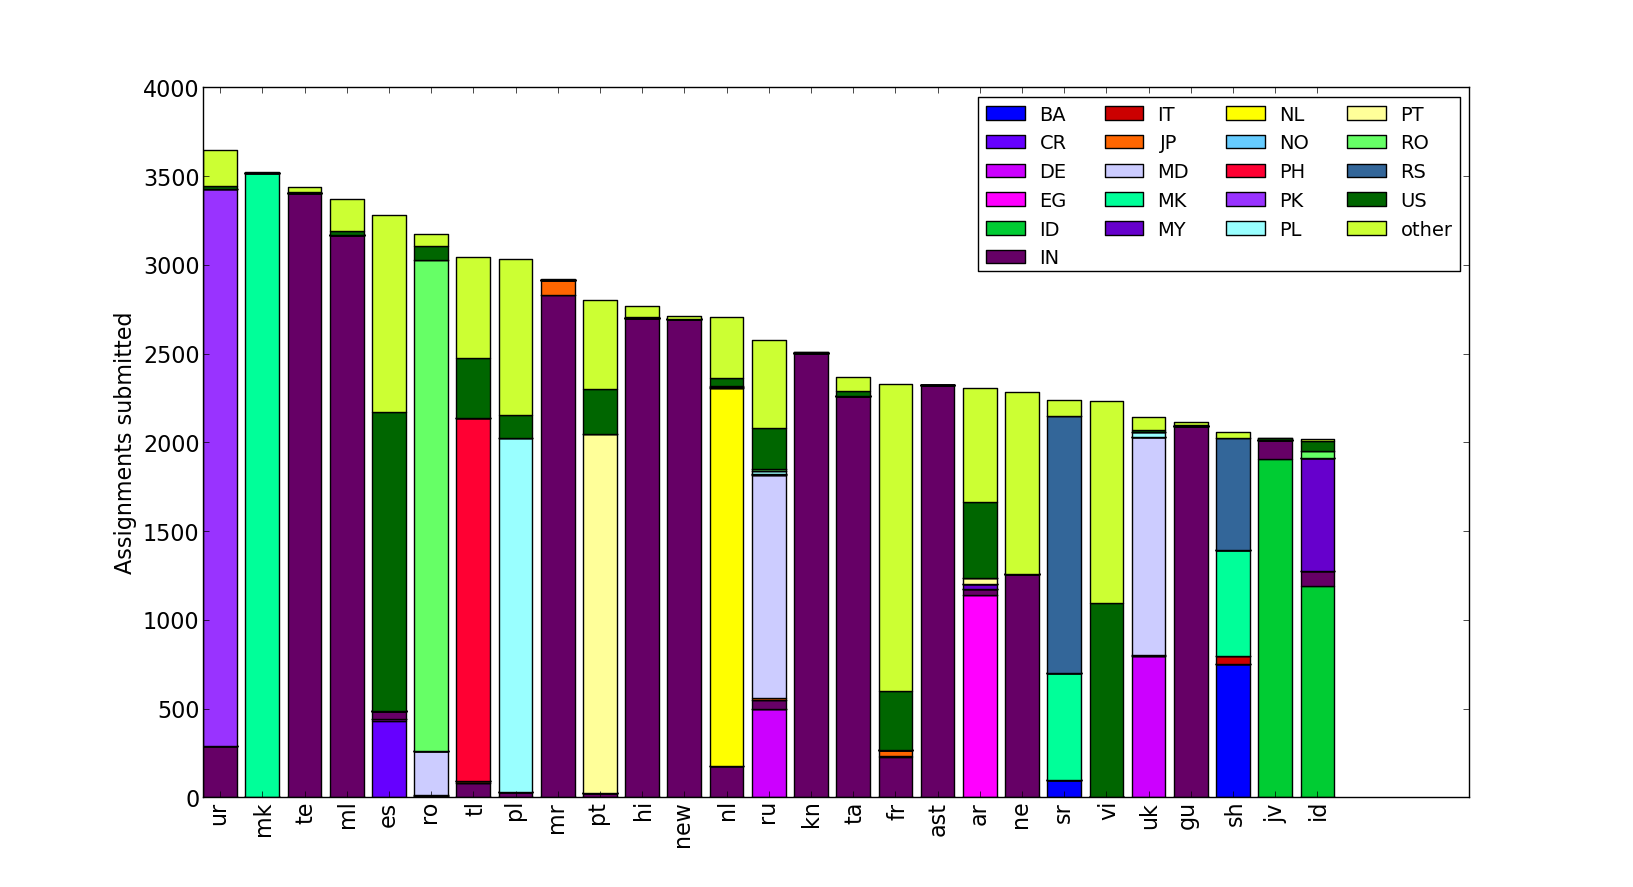
\includegraphics[width=6in]{figures/assign-langgeo-sorted}
\caption{Geolocation of turkers speaking 40 most represented languages, in terms of number of assignments submitted}
\label{langgeo-bar}
\end{figure*}
%%%%%%%%%%%%%%%%%%%%%%%%%%%%%%%%%%%%%%%%%%%%%%%%%%%%%%%%

\section{Measuring Data Quality}
The primary challenge of using crowdsourced language data is the widely variable quality of the collected annotations. While it is possible to strengthen the signal by collecting redundant labels, this strategy becomes difficult in practice for more complex data annotation. In the case of translation, even professional translations can be expected to vary significantly, and fully automatic comparison of free form text is itself an open research question.

 
In order to address the quality of the translations we received on the dictionary task, we constructed a pipeline in which the output of the translation HIT was reviewed by humans in a second evaluation HIT, described above. We quantified the quality of each translation assignment based on the output of the evaluation HIT. The quality of an assignment was scored as the fraction of known words which were acceptably translated: i.e, the supplied translation was judged to be synonymous with the gold standard translation. Since each assignment had either one or two known words embedded, each assignment was assigned a score of either 0, 0.5, or 1.


%%%%%%%%%%%%%%% MISREPORT TABLE %%%%%%%%%%%
\begin{figure}[h]
\centering
\begin{tabular}{cccc}\hline\hline\\
&Avg. & 99\%&\\
&Quality & Conf. Int.&n\\
Misreport&0.252&(0.244, 0.260)&10,479\\
Correct&0.282&(0.280, 0.283)&296,911\\
Overall&0.281&(0.279, 0.282)&307,390\\
\hline\hline
\end{tabular}
\label{mism-tab}
\caption{Quality of translations recieved from truthful versus misreporting Turkers.}
\end{figure}
%%%%%%%%%%%%%%%%%%%%%%%%%%%%%%%%%%%%%%%%%%%%%%%%%%%%%%%%

%%%%%%%%%%%%%%% HITLANG QUALITY BAR %%%%%%%%%%%
\begin{figure*}[h]
\centering
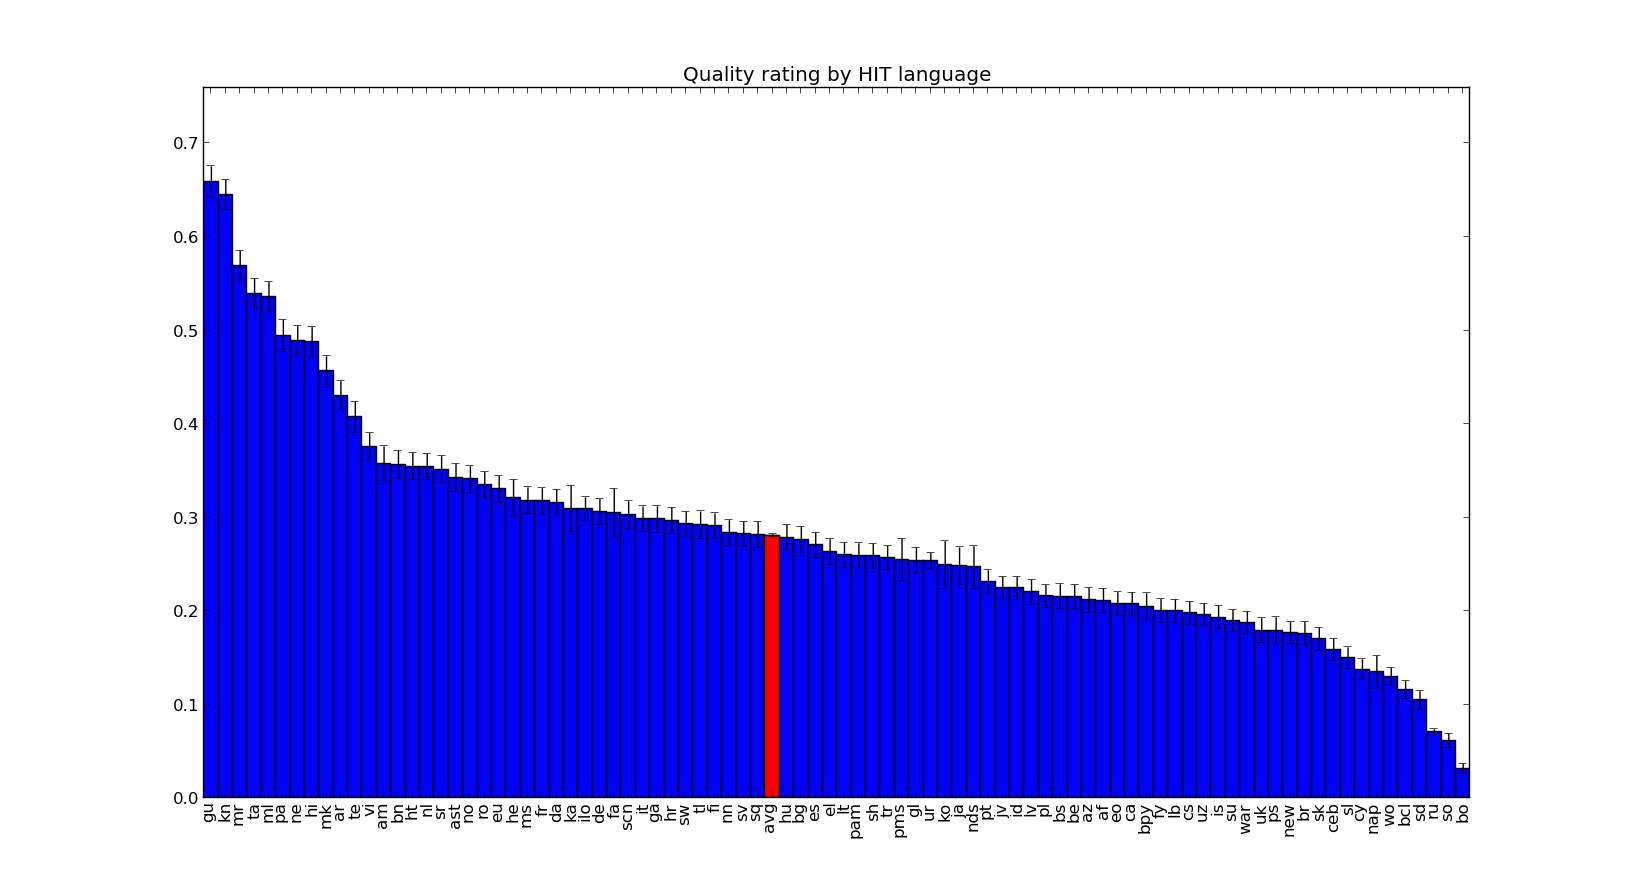
\includegraphics[width=6in]{figures/quality-hitlang}
\caption{Translation quality of by source language}
\label{hitlangqual-bar}
\end{figure*}
%%%%%%%%%%%%%%%%%%%%%%%%%%%%%%%%%%%%%%%%%%%%%%%%%%%%%%%%

Measured in this way, the average quality score across all HITs was just under 0.3. In general, countries which produced more translations did not produce lower quality translations, with India, Macedonia, and the US falling very close to average quality (figure \ref{quality-scatter}). In fact, likely as a result of the large number of India-based Turkers, most of the Indian languages fall above average quality, including Hindi, Telugu, Malayalam, Marathis, Tamil, Gujarati, Kannada, Bengali, and Punjabi, shown in figure \ref{hitlangqual-bar}. The notable exception is Urdu, which produced below average translations, likely due to the relatively low number of unique translators, making quality more susceptible to individual careless workers (see figure \ref{ass-scatter}). 


%%%%%%%%%%%%%%% NATIVE LANGUAGE QUALITY BAR %%%%%%%%%%%
\begin{figure*}[h]
\centering
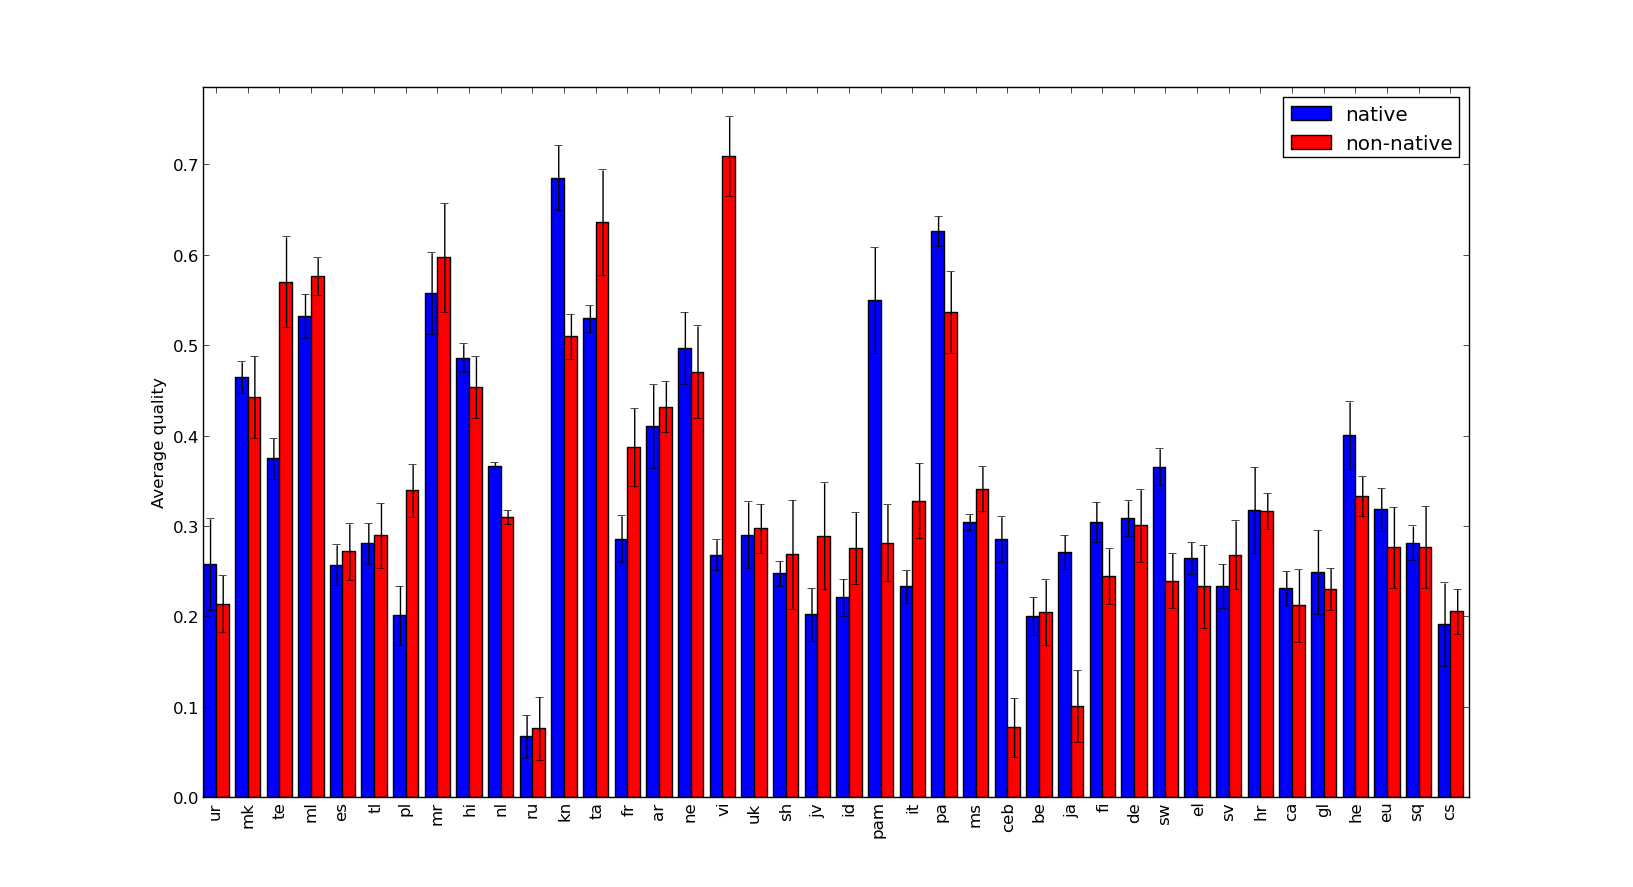
\includegraphics[width=6in]{figures/quality-natlang-sorted}
\caption{Translation quality of native and non-native speakers}
\label{natlangqual-bar}
\end{figure*}
%%%%%%%%%%%%%%%%%%%%%%%%%%%%%%%%%%%%%%%%%%%%%%%%%%%%%%%%

Interestingly, native speakers do not consistently outperform non-native speakers (see figure \ref{natlangqual-bar}). In certain unique cases, such as Vietnam, non-native speakers produce significantly better translations than native speakers, possibly due to a large population of fluent US-based workers (figure \ref{langgeo-bar}). In general, the quality difference between native and non-native speakers is not significant.	


%%%%%%%%%%%%%%% QUALITY / NUM ASSIGN SCATTER %%%%%%%%%%%
\begin{figure*}[h]
\centering
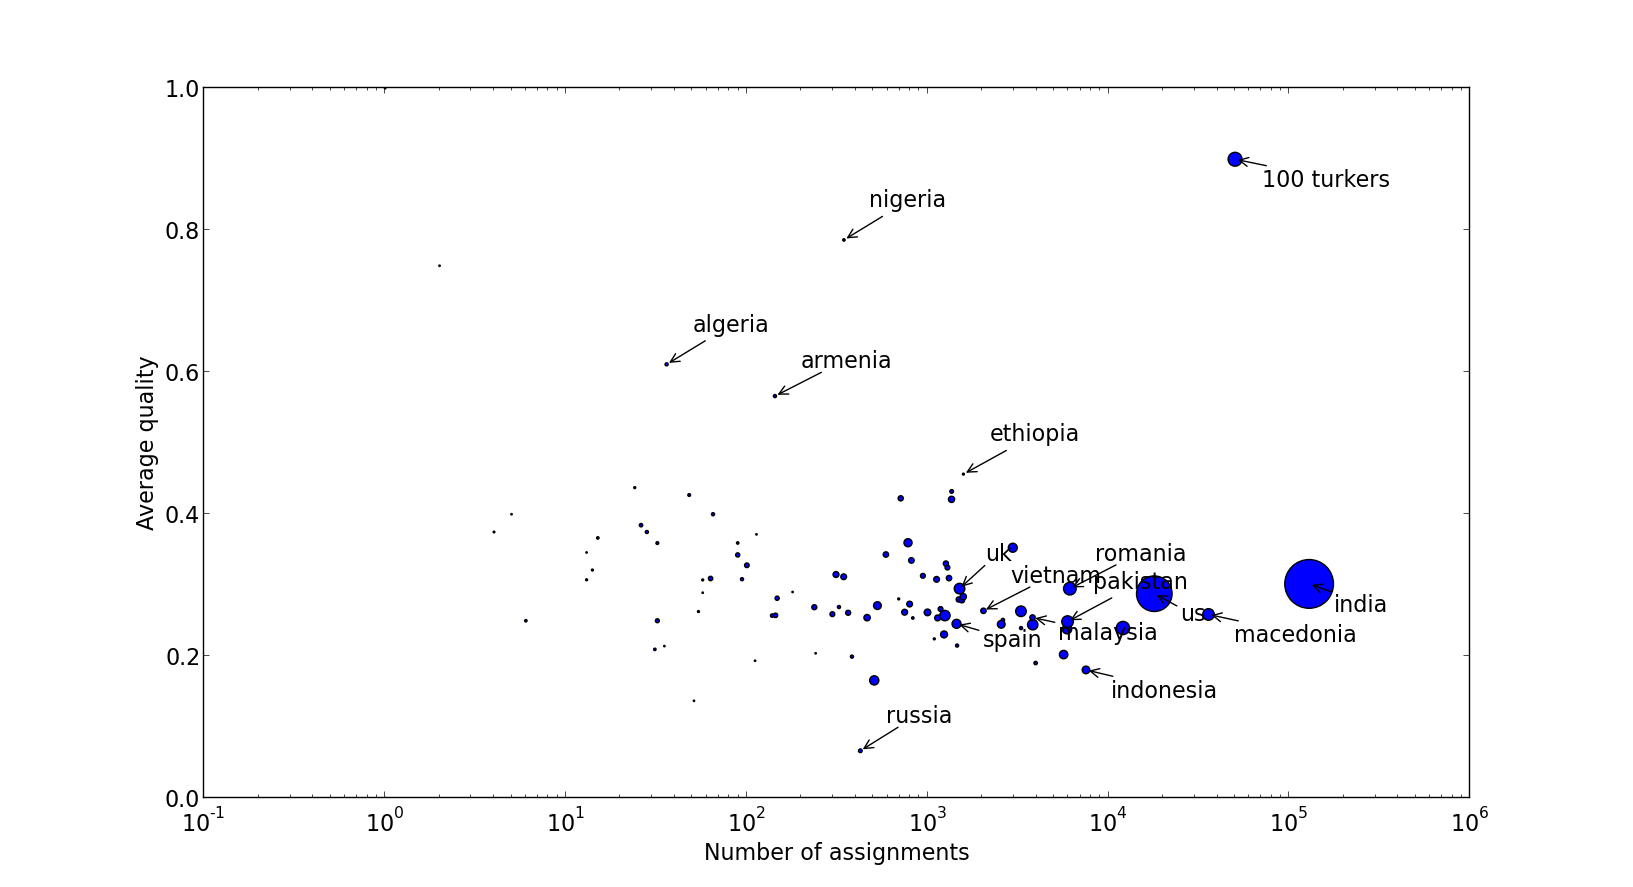
\includegraphics[width=6in]{figures/quality-scatter-avgturkers-country-labeled}
\caption{Quality of translations by country. Each circle is a country, sized proportional to the number of active Turkers from that country.}
\label{quality-scatter}
\end{figure*}
%%%%%%%%%%%%%%%%%%%%%%%%%%%%%%%%%%%%%%%%%%%%%%%%%%%%%%%%

Self-reported country information is typically reliable. Three quarters of Turkers who reported their native language reported a single native language consistantly across all assignments (table \ref{numlangs-tab}), and of those reporting multiple native languages, the majority listed English in addition to the HIT's source language, meaning less than 5\% of Turkers gave unreasonable responses. Across all assignments, 96\% of reported locations agreed with automatically reported locations, although assignments in which Turkers misreported their location averaged 10\% lower in quality than those in which the reported location was accurate, shown in table \ref{mism-tab}.


\section{Discussion}
MTurk has a strong and diverse presence of bilingual workers, making it a promising resource for researchers and developers of multilingual systems. Although unfiltered data can contain large amounts of noise, crowdsourced pipelines, which contain human oversight as a means of evaluation, offer a feasible way of ensuring high quality data, even on tasks which require more complex labels. While MTurk does offer the ability to restrict workers based on country, embedded per-task controls which are checked either automatically when possible, or manually in a second-pass HIT, are likely to provide higher quality data than naive demographic filters. 

Although our research targeted bilingual workers on Mechanical Turk, and neglected monolingual workers, we believe our results reliably represent the current speaker populations, since the vast majority of the work available on the crowdsourced platform is currently English-only.  We therefore assume the number of non-English speakers is small.  In the future, it may be desirable to recruit monolingual foreign workers.  In such cases, we recommend other tests to validate their language abilities in place of our translation test.  These could include performing narrative cloze, or listening to audio files containing speech in different language and identifying their language. 


\bibliographystyle{acl2012}
\bibliography{mturk}

\end{document}
